\documentclass[]{article}
\usepackage{lmodern}
\usepackage{amssymb,amsmath}
\usepackage{ifxetex,ifluatex}
\usepackage{fixltx2e} % provides \textsubscript
\ifnum 0\ifxetex 1\fi\ifluatex 1\fi=0 % if pdftex
  \usepackage[T1]{fontenc}
  \usepackage[utf8]{inputenc}
\else % if luatex or xelatex
  \ifxetex
    \usepackage{mathspec}
    \usepackage{xltxtra,xunicode}
  \else
    \usepackage{fontspec}
  \fi
  \defaultfontfeatures{Mapping=tex-text,Scale=MatchLowercase}
  \newcommand{\euro}{€}
\fi
% use upquote if available, for straight quotes in verbatim environments
\IfFileExists{upquote.sty}{\usepackage{upquote}}{}
% use microtype if available
\IfFileExists{microtype.sty}{%
\usepackage{microtype}
\UseMicrotypeSet[protrusion]{basicmath} % disable protrusion for tt fonts
}{}
\usepackage[margin=1in]{geometry}
\usepackage{graphicx}
\makeatletter
\def\maxwidth{\ifdim\Gin@nat@width>\linewidth\linewidth\else\Gin@nat@width\fi}
\def\maxheight{\ifdim\Gin@nat@height>\textheight\textheight\else\Gin@nat@height\fi}
\makeatother
% Scale images if necessary, so that they will not overflow the page
% margins by default, and it is still possible to overwrite the defaults
% using explicit options in \includegraphics[width, height, ...]{}
\setkeys{Gin}{width=\maxwidth,height=\maxheight,keepaspectratio}
\ifxetex
  \usepackage[setpagesize=false, % page size defined by xetex
              unicode=false, % unicode breaks when used with xetex
              xetex]{hyperref}
\else
  \usepackage[unicode=true]{hyperref}
\fi
\hypersetup{breaklinks=true,
            bookmarks=true,
            pdfauthor={Carlos Espino García},
            pdftitle={Regression Models Project},
            colorlinks=true,
            citecolor=blue,
            urlcolor=blue,
            linkcolor=magenta,
            pdfborder={0 0 0}}
\urlstyle{same}  % don't use monospace font for urls
\setlength{\parindent}{0pt}
\setlength{\parskip}{6pt plus 2pt minus 1pt}
\setlength{\emergencystretch}{3em}  % prevent overfull lines
\setcounter{secnumdepth}{5}

%%% Use protect on footnotes to avoid problems with footnotes in titles
\let\rmarkdownfootnote\footnote%
\def\footnote{\protect\rmarkdownfootnote}

%%% Change title format to be more compact
\usepackage{titling}

% Create subtitle command for use in maketitle
\newcommand{\subtitle}[1]{
  \posttitle{
    \begin{center}\large#1\end{center}
    }
}

\setlength{\droptitle}{-2em}
  \title{Regression Models Project}
  \pretitle{\vspace{\droptitle}\centering\huge}
  \posttitle{\par}
  \author{Carlos Espino García}
  \preauthor{\centering\large\emph}
  \postauthor{\par}
  \predate{\centering\large\emph}
  \postdate{\par}
  \date{July 23, 2015}



\begin{document}

\maketitle


\section{Overview}

The purpose of this project is to analyze a data set of a collection of
cars, and explore the relationship between a set of variables and miles
per gallon. We are particularly interested in answering two questions:
1. Is an automatic or manual transmission better for MPG? 2. Quantify
the MPG difference between automatic and manual transmissions

\section{Dataset}

The data was extracted from the 1974 Motor Trend US magazine, and
comprises fuel consumption and 10 aspects of automobile design and
performance for 32 automobiles (1973--74 models). The 11 variables are
the following:

\begin{enumerate}
\def\labelenumi{\arabic{enumi}.}
\itemsep1pt\parskip0pt\parsep0pt
\item
  \textbf{mpg} Miles/(US) gallon
\item
  \textbf{cyl} Number of cylinders
\item
  \textbf{disp} Displacement (cu.in.)
\item
  \textbf{hp} Gross horsepower
\item
  \textbf{drat} Rear axle ratio
\item
  \textbf{wt} Weight (lb/1000)
\item
  \textbf{qsec} 1/4 mile time
\item
  \textbf{vs} V/S
\item
  \textbf{am} Transmission (A = automatic, M = manual)
\item
  \textbf{gear} Number of forward gears
\item
  \textbf{carb} Number of carburetors
\end{enumerate}

\section{Exploratory Analysis}

To see the influence of the variables, especifically the transmission,
in the miles per gallon, Figure \ref{fig:cor_matrix} shows a matrix that
illustrates the relation of the variables. We can appreciate that disp,
hp, drat and wt have a strong linear correlation with mpg. We can
appreciate as well, that the transmission seems to influence mpg, since
the distribution of mpg is clearly divided by the type of transimission,
we can see it more clearly in Figure \ref{fig:mpg_by_trans}.

\section{Regression Analysis}

To determine wich variables influence mpg and wether or not the
transmission is important, we proceed to perform a regression analysis.

\subsection{Model Selection}

We first need to determine the method to use to select the ``best''
model. We are going choose the model by AIC in a backwards stepwise
algorithm.

The Akaike Information Criteria (AIC) is a commonly used statistic to
measures the relative goodness of fit. The AIC is a way of comparing
different models against each other.

The backwards stepwise algorithm consists in the following:

\begin{enumerate}
\def\labelenumi{\arabic{enumi}.}
\itemsep1pt\parskip0pt\parsep0pt
\item
  Start with all candidate variables.
\item
  Test the deletion of each variable using a chosen model comparison
  criterion, in this case the AIC criterion.
\item
  Delete the variable (if any) that improves the model the most by being
  deleted.
\item
  Repeat this process until no further improvement is possible.
\end{enumerate}

To perform the analysis, we take the transmission level ``Automatic''
(A) as the base level for the variable am. We define the variable
\(amM = I_{am=M}\).

After following the last steps, we get the following model.

\[\mbox{mpg} = 9.62 - 3.92\mbox{wt} + 1.23\mbox{qsec} + 2.94\mbox{amM} + \epsilon \]

The summary of the coefficients is shown in the next table

\begin{table}[ht]
\centering
\begin{tabular}{rrrrr}
  \hline
 & Estimate & Std. Error & t value & Pr($>$$|$t$|$) \\ 
  \hline
(Intercept) & 9.6178 & 6.9596 & 1.38 & 0.1779 \\ 
  wt & -3.9165 & 0.7112 & -5.51 & 0.0000 \\ 
  qsec & 1.2259 & 0.2887 & 4.25 & 0.0002 \\ 
  amM & 2.9358 & 1.4109 & 2.08 & 0.0467 \\ 
   \hline
\end{tabular}
\end{table}

\textbf{The steps of the model selection are not shown due to limitations of space}

\subsection{Coefficient Interpretation}

We can interpret the coefficient as follows: 1. For each additional 1000
lbs. of weight, the miles per gallon decrease in 3.92. 2. If each
quarter mile increase, the miles per gallon increase in 1.22. 3. The
manual transmission increases the miles per gallon in 2.94 in average
from the automatic transmission.

\subsection{Residual Analysis}

We need to perform a residual analysis to prove the assumptions of
regression analysis. Figure \ref{residuals_plot} shows some plots that
help for this analysis. We can see in the QQ-plot that the quantiles of
th residuals against the theoretical residual approximately follow the
reference line. The assumption of homoscedastic seems to be followed. We
can appreciate as well that Fiat 128, Toyota Corolla and Chrysler
Imperial are outlyers and need a deeper analysis.

\section{Conclusion}

According to the model selection criteria used, the variables wt, qsec
and am are the most important to explain mpg.
\textbf{We saw that the manual transmission is better for the performance of the car as it increases its miles per gallon in 2.94.}

\begin{figure}

{\centering 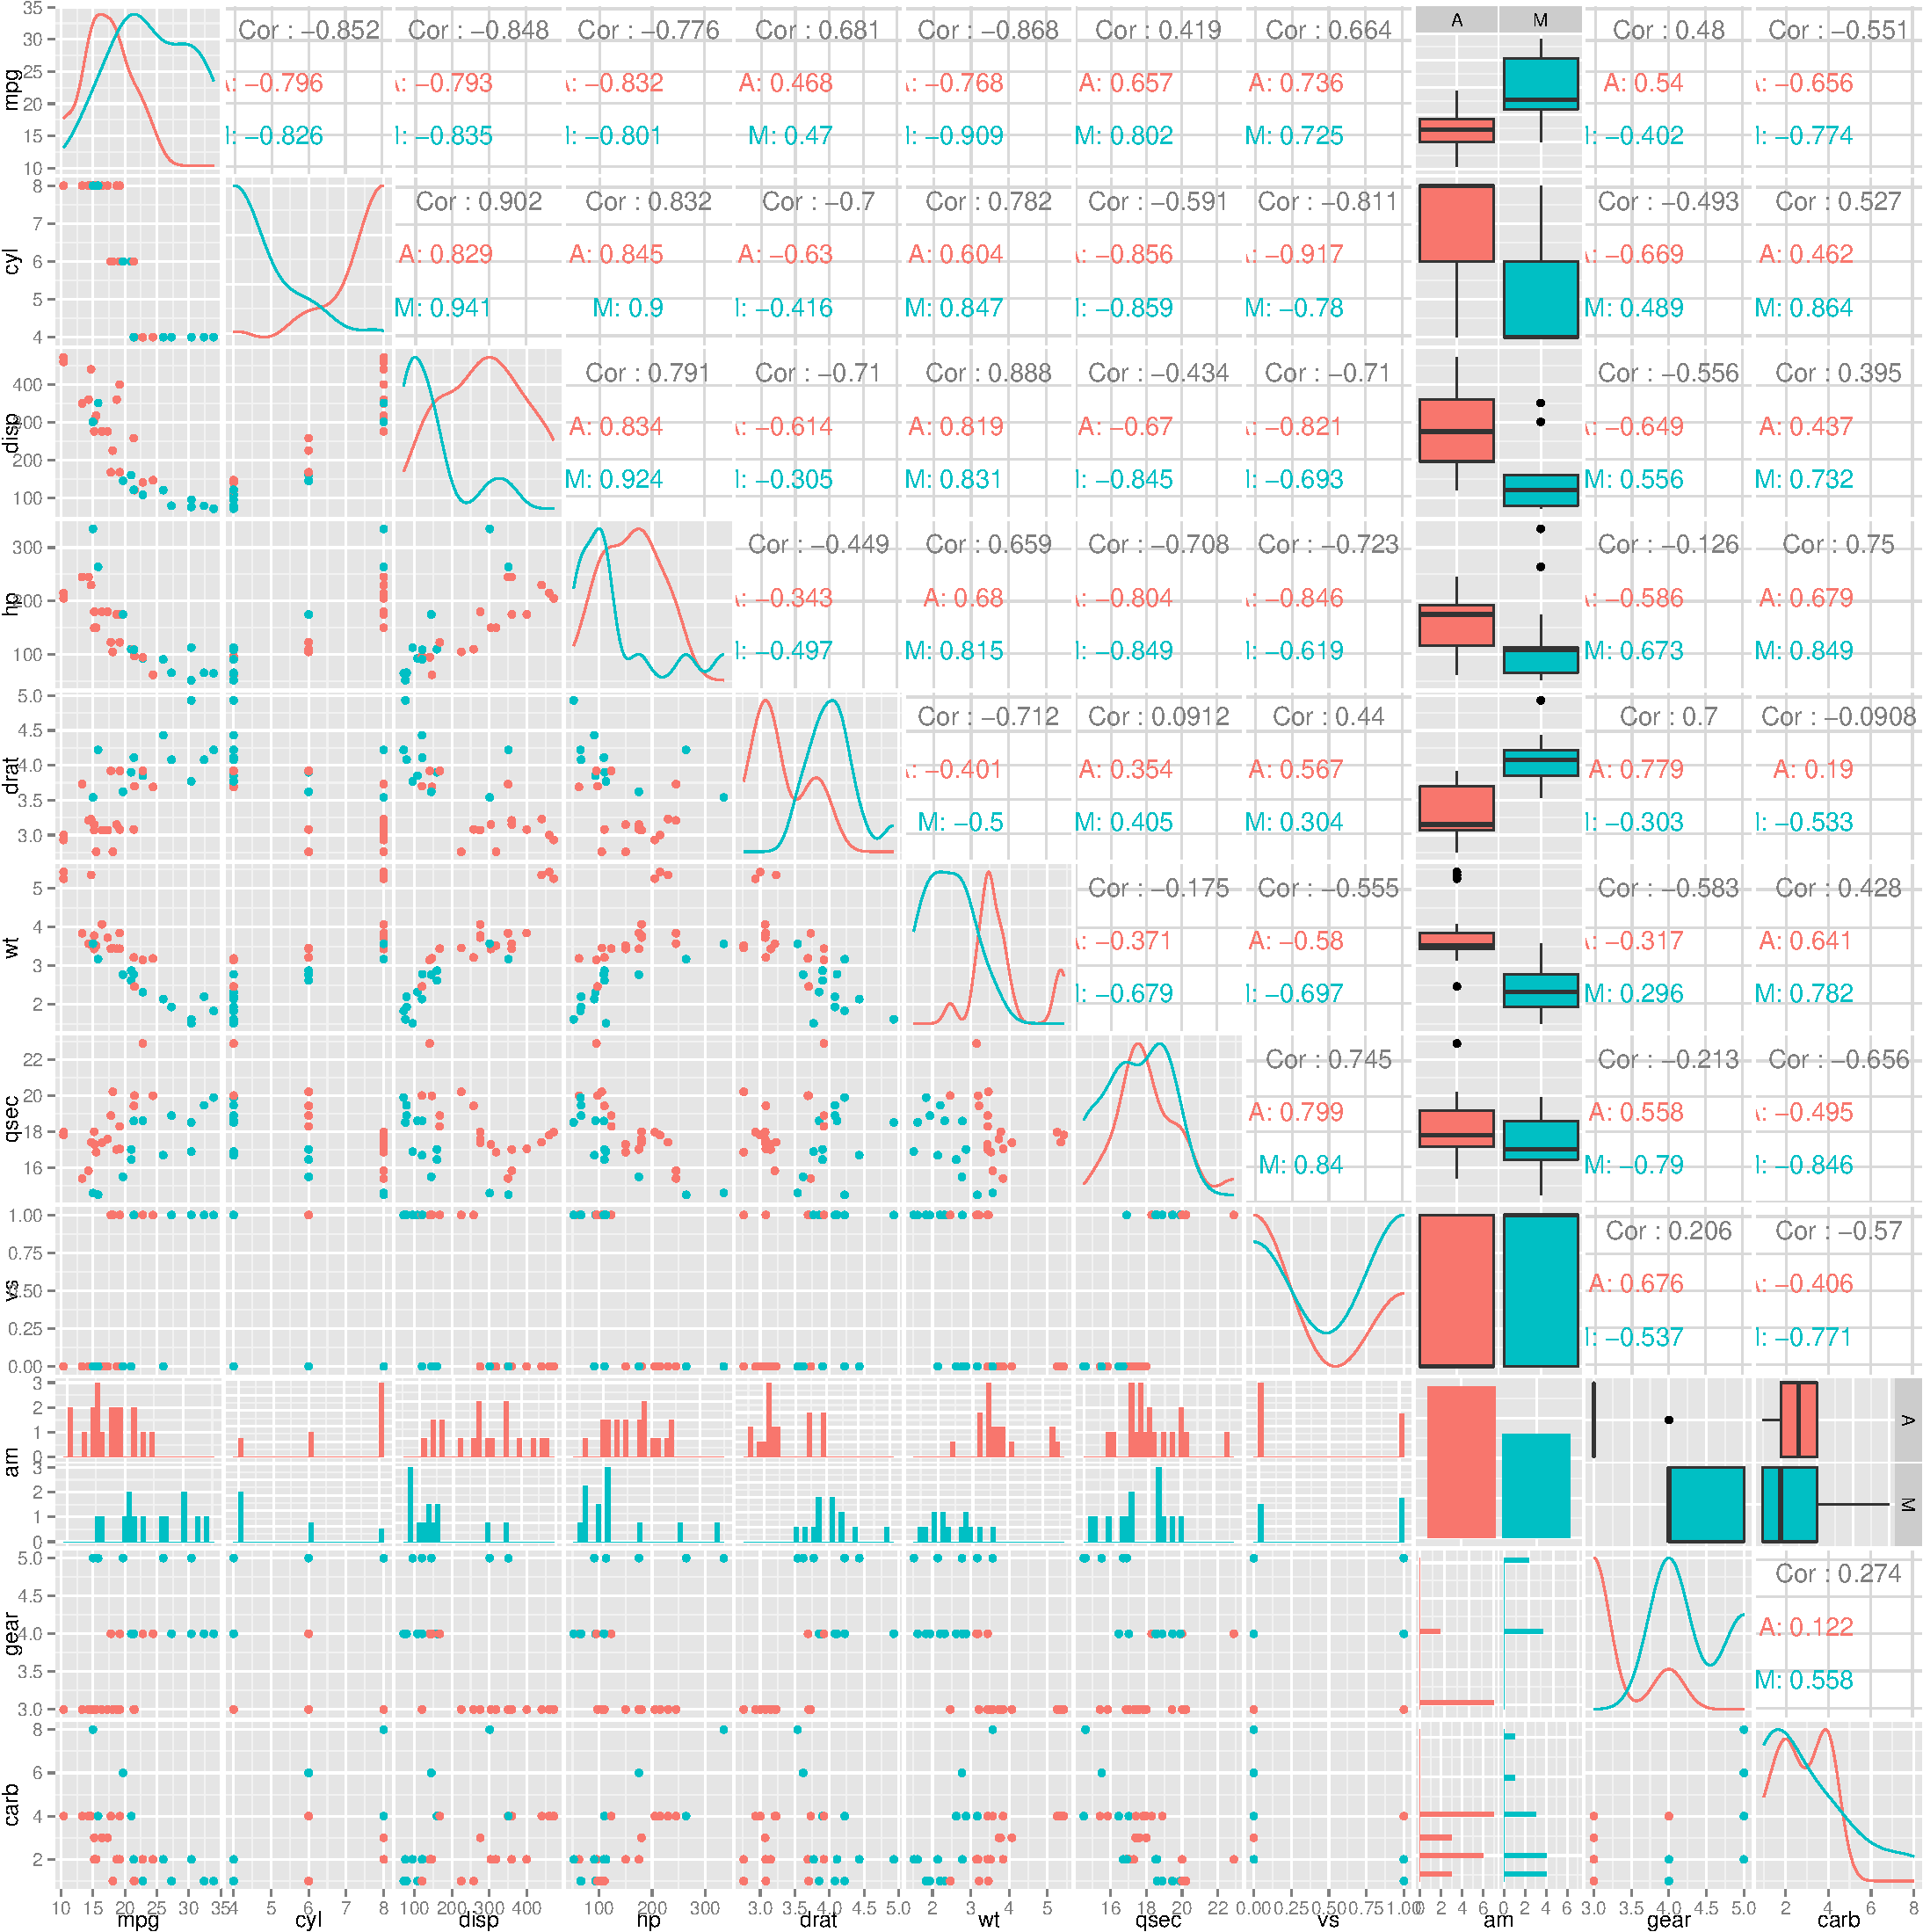
\includegraphics{Regression_Models_Project_files/figure-latex/cor_matrix-1} 

}

\caption{Correlations by transmission}\label{fig:cor_matrix}
\end{figure}

\begin{figure}

{\centering 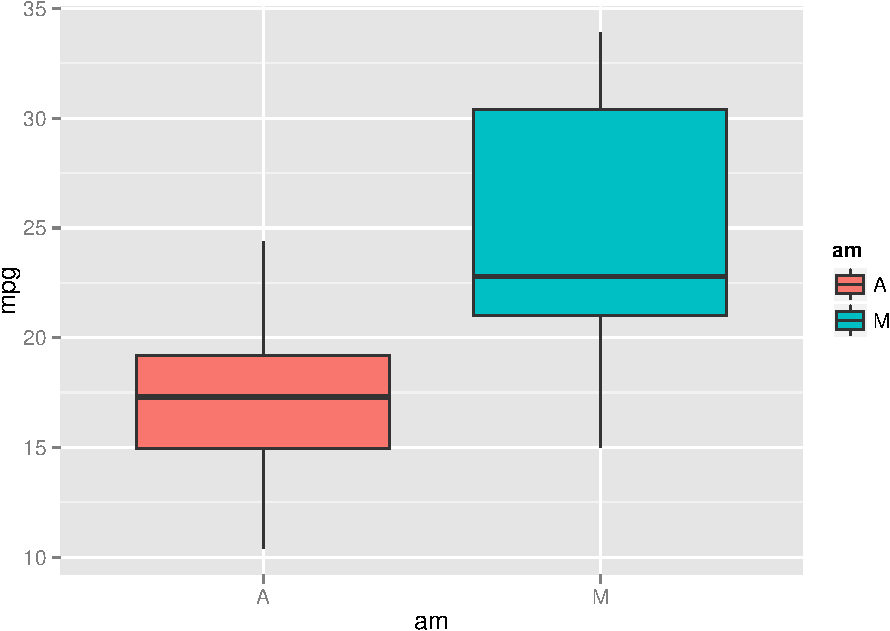
\includegraphics[width=.6\textwidth]{Regression_Models_Project_files/figure-latex/mpg_by_trans-1} 

}

\caption{mpg by transmission}\label{fig:mpg_by_trans}
\end{figure}

\begin{figure}[htbp]
\centering
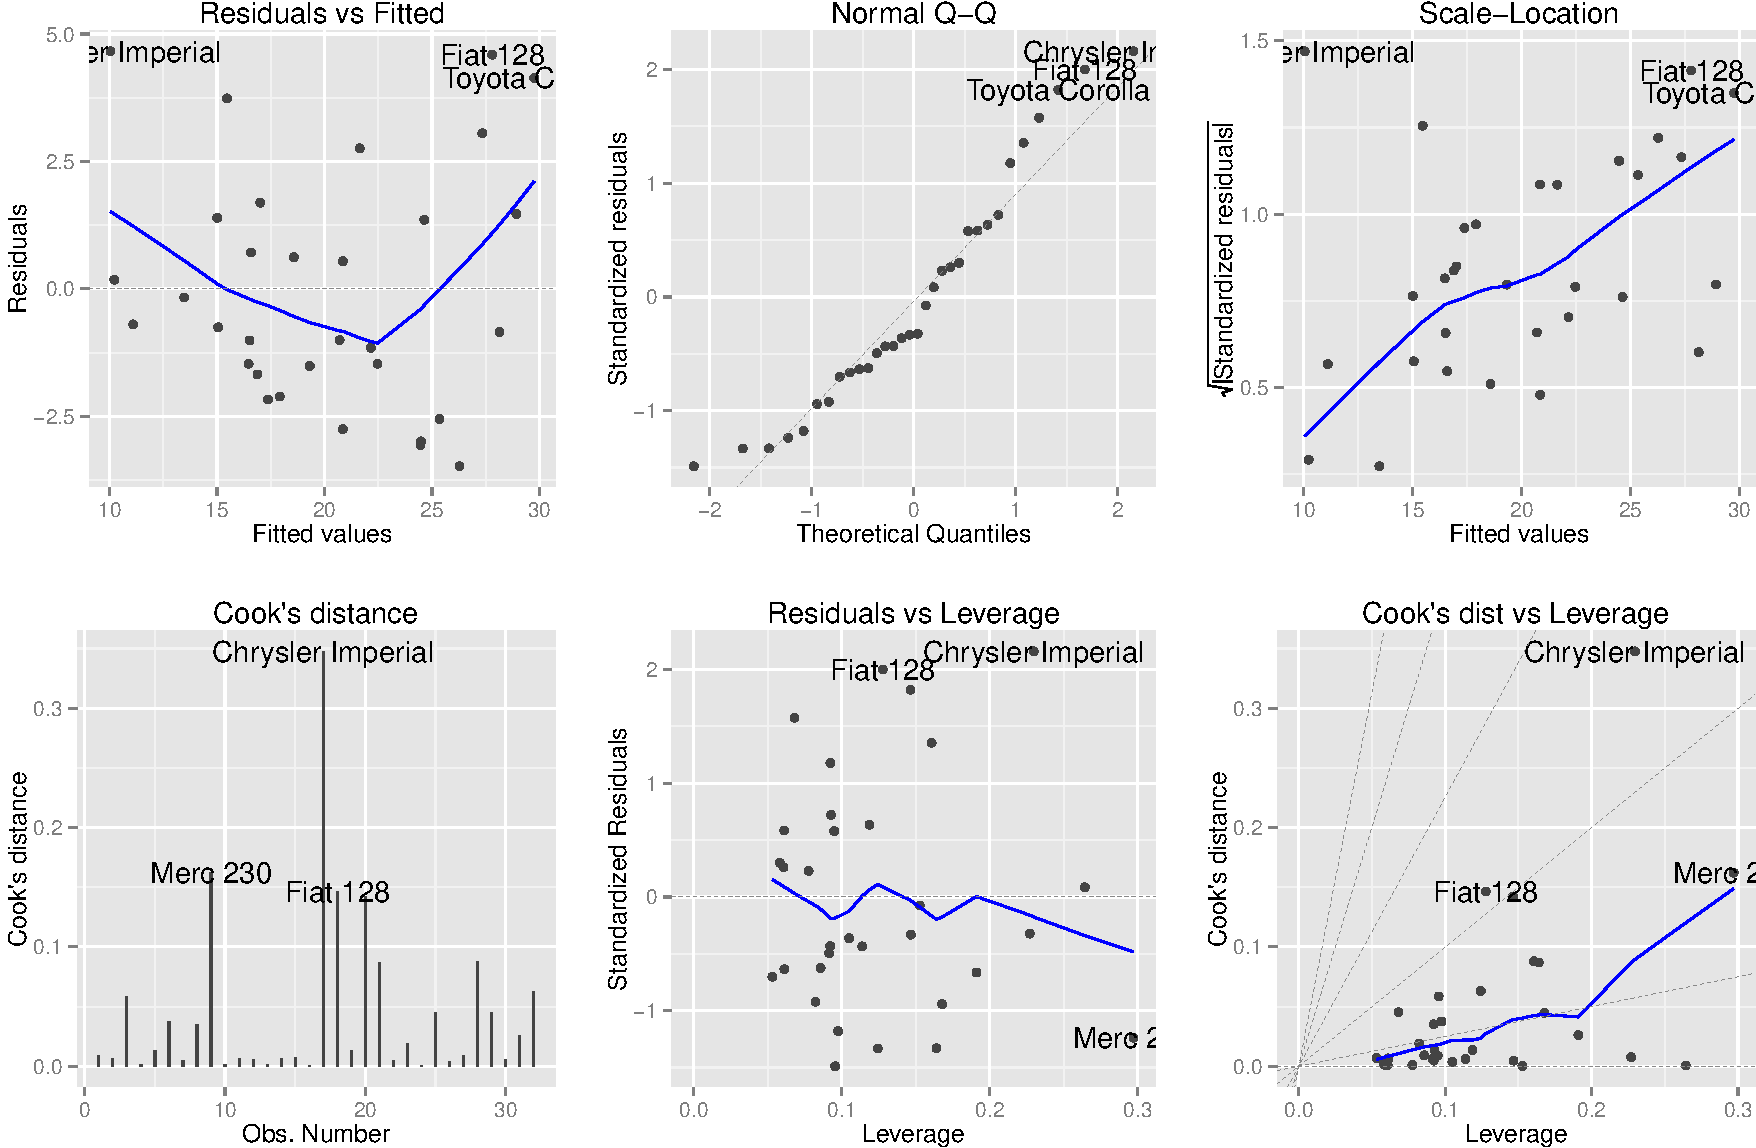
\includegraphics{Regression_Models_Project_files/figure-latex/residuals_plot-1.pdf}
\caption{Residual analysis plots}
\end{figure}

\end{document}
